\section{Modello di sviluppo}
Per lo sviluppo del progetto \textit{Etherless} abbiamo deciso di adottare il \textbf{modello incrementale}.

	\subsection{Modello incrementale}
	\begin{figure}[h!]
		\centering
		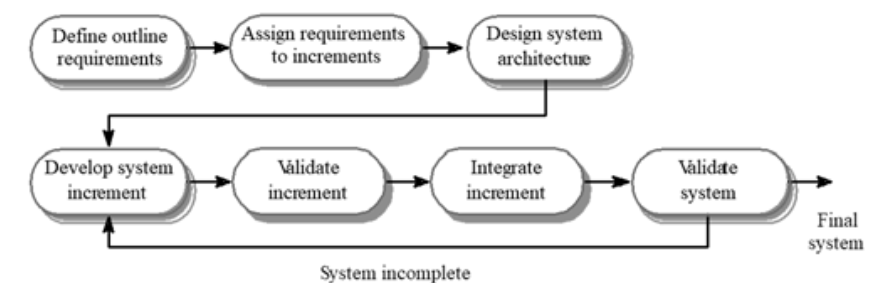
\includegraphics[width=0.9\textwidth]{./res/img/modello_incr.png}
		\caption{Rappresentazione del modello incrementale}
	\end{figure}

	L'adottarsi di un modello di sviluppo incrementale implica lo sviluppo del prodotto\ped{\textit{G}} tramite multipli rilasci successivi, ognuno dei quali implementa una nuova funzionalità che viene incorporata nel sistema. Questi rilasci sono detti appunto "incrementi". Il numero di incrementi e le funzionalità da implementare all'interno di ognuno sono identificati a partire dai requisiti esposti dal Proponente\ped{\textit{G}} e analizzati dal gruppo \Gruppo{}. Gli incrementi sono ordinati in modo da iniziare con quelli che contengono funzionalità a priorità più alta. All'inizio di ogni incremento si descrivono in dettaglio i requisiti che verranno soddisfatti con il suo completamento, per poi procedere con lo sviluppo. L'incremento viene quindi aggiunto al prodotto\ped{\textit{G}} e si procede con l'incremento successivo. Per garantire l'efficacia del modello di sviluppo, durante la fase di sviluppo non sono permesse modifiche dei requisiti, a meno che questi non vadano soddisfatti durante incrementi successivi.\\
	Il modello incrementale è stato ritenuto preferibile considerando i seguenti vantaggi:

	\begin{itemize}
		\item ogni incremento porta un valore aggiunto, spingendo verso un avanzamento continuo del progetto;
		\item sviluppo delle funzionalità più importanti all'inizio grazie all'ordinamento degli incrementi;
		\item i requisiti più importanti vengono chiariti negli stadi iniziali della realizzazione del prodotto\ped{\textit{G}};
		\item l'uso di questo modello di sviluppo favorisce lo sviluppo di prototipi funzionanti, che a loro volta favoriscono la validazione dei requisiti e la comunicazione con il Proponente\ped{\textit{G}}.
	\end{itemize}

	\subsection{Incrementi pianificati}
	Si prevede di svolgere 23 incrementi con il fine di integrare tutte le funzionalità richieste dal progetto. Di seguito si riporta una tabella riassuntiva degli incrementi, con una breve descrizione sul relativo svolgimento e i requisiti che vengono soddisfatti. \\
	I requisiti riportati includono anche tutti i requisiti figli. Tutti i requisiti non riportati nella tabella sono da intendersi soddisfatti in parte da ogni incremento. 
	
	\rowcolors{2}{lightRowColor}{darkRowColor}
	\begin{longtable}{
			>{\centering}p{0.2\textwidth}	%
			>{\centering}p{0.35\textwidth}	%
			>{\centering}p{0.35\textwidth}	%
		 }	
		
		\coloredTableHead
		\textbf{\color{white}Incremento} &
		\textbf{\color{white}Obiettivi} &
		\textbf{\color{white}Requisiti}
		\tabularnewline
		\endhead
		
		1$^{\circ}$ incremento & Integrazione dei documenti a seguito delle conoscenze acquisite nei periodi precedenti. & Non saranno aggiunte nuove funzionalità software. \tabularnewline
		2$^{\circ}$ incremento & Creazione della componente \textit{Etherless-smart} e gestione delle richieste di esecuzione. & Parziale R1F9. \tabularnewline
		3$^{\circ}$ incremento & Creazione della componente \textit{Etherless-cli} e delle funzionalità di autenticazione, registrazione e richiesta di esecuzione di una funzione. & R1F3, R1F4, R1F5, parziale R1F9. \tabularnewline
		4$^{\circ}$ incremento & Creazione della componente \textit{Etherless-server} e completamento della gestione dell'esecuzione di una funzione. & Parziale R1F9. \tabularnewline
		5$^{\circ}$ incremento & Integrazione delle tre componenti sviluppate. & Completamento R1F9. \tabularnewline
		6$^{\circ}$ incremento & Correzione della documentazione a seguito della RR e preparazione della \textit{Technology Baseline}. & Non saranno aggiunte nuove funzionalità software. \tabularnewline
		7$^{\circ}$ incremento & Ulteriori aggiornamenti della documentazione, con passaggio alla versione 2.0.0. & Non saranno aggiunte nuove funzionalità software. \tabularnewline
		8$^{\circ}$ incremento  & Preparazione alla presentazione RP. & Non saranno aggiunte nuove funzionalità software. \tabularnewline
		9$^{\circ}$ incremento & Correzione dei documenti a seguito delle conoscenze acquisite nei periodi precedenti. & Non saranno aggiunte nuove funzionalità software. \tabularnewline
		10$^{\circ}$ incremento & Scelta dell'architettura da applicare al prodotto software. & Non saranno aggiunte nuove funzionalità software. \tabularnewline
		11$^{\circ}$ incremento & Adattamento delle componenti già sviluppate all'architettura scelta. & Non saranno aggiunte nuove funzionalità software. \tabularnewline
		12$^{\circ}$ incremento & Implementazione della funzionalità di rilascio di una nuova funzione. & R1F11. \tabularnewline
		13$^{\circ}$ incremento  & Implementazione della funzionalità di eliminazione di una funzione. & R1F14. \tabularnewline
		14$^{\circ}$ incremento & Implementazione delle funzionalità per ottenere informazioni riguardo alla funzioni disponibili nella piattaforma. & R1F7, R1F10. \tabularnewline
		15$^{\circ}$ incremento & Stesura dei manuali e aggiornamento della documentazione. & Non saranno aggiunte nuove funzionalità software. \tabularnewline
		16$^{\circ}$ incremento & Preparazione della presentazione per la RQ e conseguente raffinamento della demo. & Non saranno aggiunte nuove funzionalità software. \tabularnewline
		17$^{\circ}$ incremento & Correzione ed integrazione dei documenti a seguito delle conoscenze acquisite nei periodi precedenti. & Non saranno aggiunte nuove funzionalità software. \tabularnewline
		18$^{\circ}$ incremento & Ampliamento delle funzionalità messe a disposizione del modulo \textit{Etherless-cli}; comandi: init, whoami, search. & R2F1, R2F2, R2F6, R2F8. \tabularnewline
		19$^{\circ}$ incremento & Implementazione del comando \texttt{history} all'interno del moduli \textit{Etherless-cli}. & R2F13. \tabularnewline
		20$^{\circ}$ incremento  & Implementazione della funzionalità di aggiornamento di una funzione già caricata all'interno della piattaforma. & R2F12. \tabularnewline
		21$^{\circ}$ incremento & Ampliamento dei test ed eventuali correzioni necessarie. & Non saranno aggiunte nuove funzionalità software. \tabularnewline
		22$^{\circ}$ incremento & Aggiornamento della documentazione. & Non saranno aggiunte nuove funzionalità software. \tabularnewline
		23$^{\circ}$ incremento & Preparazione della presentazione per la RA. & Non saranno aggiunte nuove funzionalità software. \tabularnewline
	\end{longtable}